\documentclass{beamer}

\usepackage{lipsum}
\usepackage[orientation=landscape,size=a0,scale=1.2]{beamerposter}
\usepackage{amsmath,amsthm, amssymb}

%\boldmath

%\title[Beamer Poster]{Overleaf example of the beamerposter class}
%\author[welcome@overleaf.com]{Overleaf Team}
%\institute[Overleaf University]
%{The Overleaf institute, Learn faculty}
%\date{\today}

\graphicspath{{images/}}
\usepackage{hyperref}
\hypersetup{
	colorlinks=true,
	linkcolor=blue,
	filecolor=magenta,      
	urlcolor=cyan,
}
%\logo{\includegraphics[height=7.5cm]{example-image-a}}
\usetheme[]{default}
\definecolor{main}{HTML}{750f6d}
%\setbeamercolor*{palette primary}{bg=white}
\definecolor{background}{RGB}{250, 250, 250}
\setbeamercolor{block title}{bg=main, fg=background}
\setbeamercolor{block body}{bg=main!1!background, fg=black}
\setbeamertemplate{caption}[numbered]

\setbeamertemplate{bibliography item}[text]

%\footlineinfo{123}
\setbeamercolor{footline}{fg=main, bg=main}  % Disable the page number
\setbeamertemplate{headline}{
	\begin{beamercolorbox}[wd=\paperwidth]{headline}
		\begin{columns}
			\begin{column}{0.125\linewidth}
				\hspace{\fill}
				\centering
				\includegraphics[width=0.85\linewidth]{cuhk-emblem}
			\end{column}
			\begin{column}{0.75\linewidth}
				\vspace{5mm}
				
				\centering\bfseries
				{\fontsize{80}{96}\selectfont Optimal Sensor Fusion using $\mathcal{H}_\infty$ methods} \\ {\fontsize{60}{72}\selectfont Synthesizing Complementary Filters for Active Seismic Noise Isolation Systems in KAGRA}\\[10mm]
				\mdseries
				{\fontsize{60}{72}\selectfont Terrence T.L. Tsang on behalf of the KAGRA Collaboration} \\[10mm]
				{\fontsize{40}{48}\selectfont The Chinese University of Hong Kong. Email: \href{mailto:ttltsang@link.cuhk.edu.hk}{ttltsang@link.cuhk.edu.hk}}
			\end{column}
			\begin{column}{0.125\linewidth}
				\centering
				
\includegraphics[width=0.85\linewidth]{KAGRA-logo}
				\hspace{\fill}
			\end{column}
		\end{columns}
	\end{beamercolorbox}
%\color{main!80!background}\rule{\paperwidth}{20pt}
}


\begin{document}
\begin{frame}[t]
%	\begin{abstract}
%		\lipsum[1]
%	\end{abstract}
	\begin{columns}[t]
		
		% Column 1
		\begin{column}{0.32\linewidth}
			
			\begin{block}{Introduction}
				Seismic isolation for ground-based interferometric gravitation-wave detectors plays a crucial  role for suppressing the displacement level of the main optics so 1) the main optics are sufficiently stable to not cause lock-loss of the interferometer, and 2) displacement noise at detection band ($>10\,\text{Hz}$) does not compromise the sensitivity of the detector.
%				\begin{enumerate}
%					\item the main optics are sufficiently stable to not cause lock-loss of the interferometer, and 
%					\item displacement noise at detection band (> 10 Hz) does not compromise the sensitivity of the detector.
%				\end{enumerate}
				\medskip
				
				\begin{columns}[t, onlytextwidth]
					\begin{column}{0.4\textwidth}	
						At higher frequencies, the displacement of the optics due to seismic noise is suppressed passively by suspending the optics with multiple-stage pendulum (suspension).
						At lower frequencies, the residual motion of the optics is dominated by resonances excited by the ground motion.
						While passive isolation is only effective at frequencies higher than the resonances, the residual motion of the optics at lower frequencies is reduced by active isolation using control systems.
					\end{column}
					\begin{column}{0.6\textwidth}
						\begin{figure}
							\centering
							\includegraphics[width=0.9\linewidth]{Suspension_types}
							\caption{Type-A suspensions: input/end test masses, Type-B suspensions: beamsplitter and signal-recycling mirrors, Type-Bp suspensions: power-recycling mirrors, and Type-C suspensions: input/output mode cleaners \cite{Akutsu:2021auw}.}
						\end{figure}
					\end{column}
				\end{columns}
				
				\medskip
				
				In particular, we're interested in using feedback systems that manipulate displacement signals from sensors and feedback to the suspension via actuators.
				While such control systems are effective in reducing the displacement level suspension at the control band, control noises are introduced at higher frequencies.
				To satisfy the displacement noise requirements, control regulators need to be roll-off, which limits the amount of attenuation from the feedback system.
				Since the control noise is dominated by sensing noise, lowering the sensing noise at higher frequencies enables the possibility of a greater control gain at lower frequencies, which makes the optics less susceptible to seismic disturbance.	
				
				\medskip
				
				Here, we will describe a sensor fusion technique, which combines multiple sensors with different noise characteristics using complementary filters.
				The combined ``super sensor'' has an overall better noise performance, which can potentially enhance suspension control performance that ultimately translates to a more stable interferometer with lower detector noise.
				This technique is used particularly for the preisolator stage, which is closest to the ground and furthest from the optics, of the Type-A and Type-B suspensions, where relative displacement sensors and inertial sensors were both used for feedback control.
				So, we will describe a method that can be used to synthesize complementary filters, using $\mathcal{H}_\infty$ method, that optimally combine two sensors.
			\end{block}
				
			\begin{block}{Methodology}
				\begin{columns}[t, onlytextwidth]
					\begin{column}{0.5\textwidth}
						Fig.~\ref{fig:two-sensor} shows a the block diagram typical two-sensor sensor fusion configuration using complementary filters.
						Note that only the noise path is shown and the signal path is omitted.
						Here, there are two sensors with sensing noises $N_1(s)$ and $N_2(s)$ and they are both sensing a common displacement signal.
						Note that $s$ is the complex variable and all variables are specified in the frequency/Laplace domain unless otherwise specified.
					\end{column}
					\begin{column}{0.5\textwidth}
						\begin{figure}
							\centering
							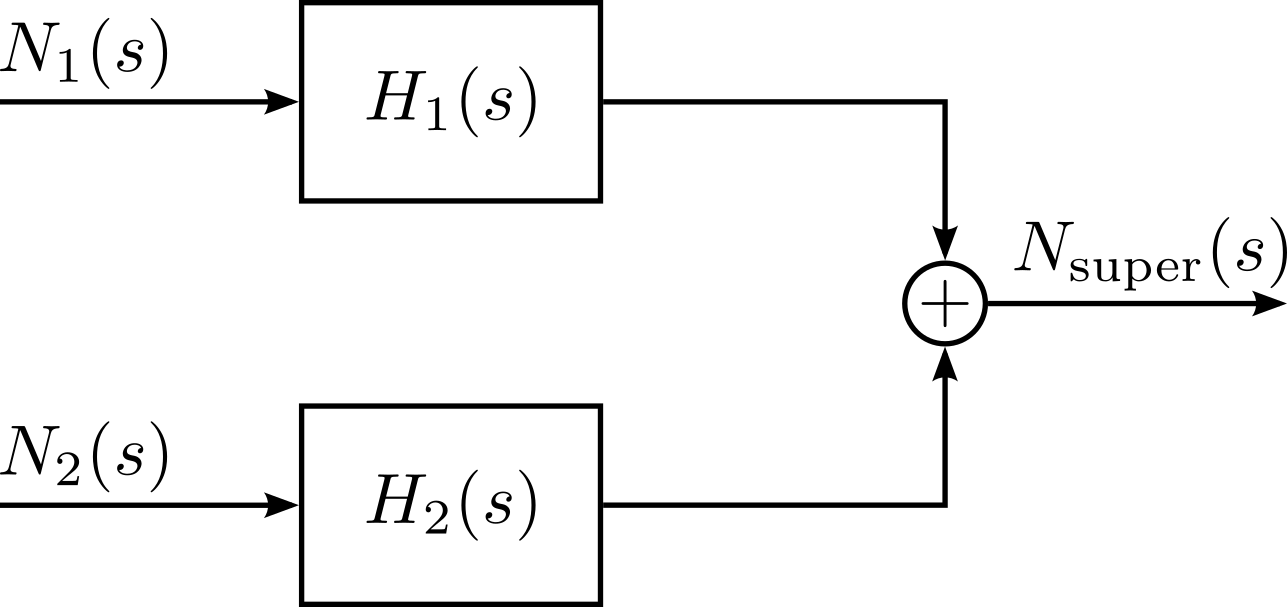
\includegraphics[width=1\linewidth]{complementary_filter}
							\caption{Two-sensor complementary filter configuration.}
							\label{fig:two-sensor}
						\end{figure}
					\end{column}
				\end{columns}
			
			\medskip
			
			The two sensors are each filtered with filters $H_1(s)$ and $H_2(s)$ respectively.
			We required that the super sensor measuring the same signal that the two sensors are reading, so the filters must be complementary, i.e.
			\begin{equation}
				H_1(s) + H_2(s) = 1\,.
				\label{eqn:complementary}
			\end{equation}
			\end{block}
		\end{column}
	
		% Column 2
		\begin{column}{0.32\linewidth}
			\begin{block}{Methodology (cont.)}
				
				The super sensor noise then reads
				\begin{equation}
					N_\text{super}(s) = H_1(s)N_1(s) + H_2(s)N_2(s)\,.
					\label{eqn:noise_super}
				\end{equation}
				So, the goal is to design the complementary filters $H_1(s)$ and $H_2(s)$ such that $N_\text{super}(s)$ is minimized in some sense, or exhibit desirable noise characteristics.
				
				\medskip
				
				In previous work, there were proposed complementary filter designs that tackles the problem by matching the frequency-dependency of the sensing noises and the roll-off of the filter \cite{Sekiguchi:2016bmv, vanHeijningen:2018cpc}.
				However, the filter shapes are too simple and is not flexible.
				Undoubtedly, it is possible to improve the noise performance by better shaping of the filters.
				Indeed, this was done in \cite{low_frequency_optimization_and_performance_of_advanced_virgo_seismic_isolation_system}, where the filter is shaped to minimize seismic noise coupling in the relative displacement sensors.
				But, this raises another problem where the filters are tuned manually by heuristics, which may suboptimal and non-reproducible due to the human factor.
				Therefore, we seek to find a method that can automatically generate optimal complementary filters according to the sensing noises themselves.
				
				\medskip
				
				\begin{columns}[t, onlytextwidth]
					\begin{column}{0.5\textwidth}
						This is where $\mathcal{H}_\infty$ method comes in.
						$\mathcal{H}_\infty$ method is used to synthesize regulator for feedback systems but is recently proposed for synthesizing complementary filters with frequency-dependent specification \cite{Thomas:2019}.
						And, It was shown that the method successfully reproduced one of the complementary filters at LIGO \cite{Matichard:2015} using the same specifications.
						To use $\mathcal{H}_\infty$ method, the input-output system is first represented in the generalized plant representation as shown in Fig.~\ref{fig:generalized_plant_representation}.
					\end{column}
					\begin{column}{0.5\textwidth}
						\begin{figure}
							\centering
							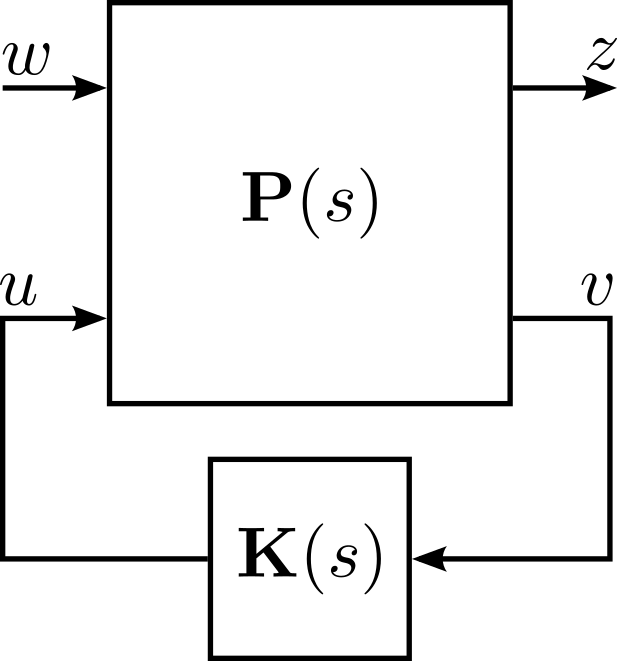
\includegraphics[width=0.55\linewidth]{generalized_plant}
							\caption{Generalized Plant Represenation}
							\label{fig:generalized_plant_representation}
						\end{figure}
					\end{column}
				\end{columns}
			
			\medskip
			
			In the figure, $w$ are the inputs, $z$ are the error signals to be minimized, $u$ are the manipulated variables, $v$ are the measurement signals, $\mathbf{P}(s)$ is the open loop plant, and $\mathbf{K}(s)$ is the closed-loop regulator.
			The close-loop response can be written as
			\begin{equation}
				z=\mathbf{G}(s)w\,,
			\end{equation}
			where $\mathbf{G}(s) = P_{11}(s) + P_{12}(s)\mathbf{K}(s)\left(I-P_{22}(s)\mathbf{K}(s)\right)^{-1}P_{21}(s)$ is the closed-loop transfer function matrix of the system.
			$\mathcal{H}_\infty$ synthesis will then generate a regulator $\mathbf{K}_\infty(s)$, which minimizes the $\mathcal{H}_\infty$ norm of the closed-loop transfer function $\mathbf{G}(s)$.
			The $\mathcal{H}_\infty$ norm of the transfer function matrix is defined by
			\begin{equation}
				\left\Vert\mathbf{G}(j\omega)\right\Vert_\infty = \sup_\omega\left(\bar\sigma(\mathbf{G}(j\omega))\right)\,,
			\end{equation}
			where $j$ denotes the imaginary number, $\omega$ is the angular frequency, $\sup$ denotes the supremum, and $\bar\sigma(\mathbf{G}(j\omega))$ is the maximum singular value of $\mathbf{G}(s)$ at $\omega$.
			
			\medskip
			
			\begin{columns}[t, onlytextwidth]
				\begin{column}{0.475\textwidth}
					Although everything about $\mathcal{H}_\infty$ method so far has been discussed under the context of feedback control, it can also be used to synthesize complementary filters.
					Consider the generalized plant architecture as shown in Fig.~\ref{fig:generlized_plant_complementary_filter}.
					Here, $\Phi_1$ and $\Phi_2$ are some uncorrelated stochastic processes with unit magnitude.
					$\hat{N}_1$ and $\hat{N}_2$ are transfer function models of the noises $N_1$ and $N_2$ such that
					$N_1(s) = \hat{N}_1(s)\Phi_1$ and $N_2(s) = \hat{N}_2(s)\Phi_2$.
					$W_1(s)$ and $W_2(s)$ are some weighting functions.
				\end{column}
				\begin{column}{0.5\textwidth}
					\begin{figure}[!h]
						\centering
						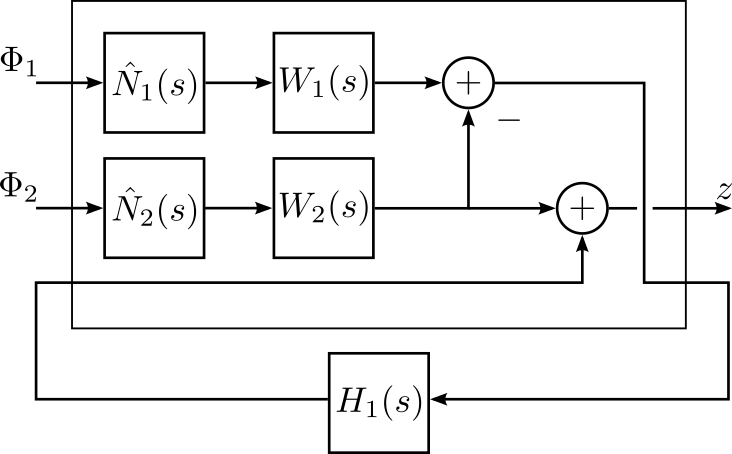
\includegraphics[width=1\linewidth]{generalized_plant_complementary_filter}
						\caption{Generalized plant representation for complementary filter synthesis.}
						\label{fig:generlized_plant_complementary_filter}
					\end{figure}
				\end{column}
			\end{columns}
		
			\medskip
			
			The closed-loop transfer function reads
			\begin{equation}
				\mathbf{G}(s) = \begin{bmatrix}H_1(s)\hat{N}_1(s)W_1(s) & H_2(s)\hat{N}_2(s)W_2(s)\end{bmatrix}\,,
			\end{equation}
			where we've substitute $(1-H_1(s))$ with $H_2(s)$ due to Eqn.~\eqref{eqn:complementary}.
			\end{block}
			
			
		\end{column}
	
		% Column 3
		\begin{column}{0.32\linewidth}
			\begin{block}{Methodology (cont.)}
				The plant has a maximum singular value of
				\begin{equation}
				\bar\sigma(\mathbf{G}(j\omega)) \approx \max{(H_1(j\omega)\hat{N}_1(j\omega)W_1(j\omega),H_2(j\omega)\hat{N}_2(j\omega)W_2(j\omega))}\,,
				\end{equation}
				Now, if we set $W_1(s)=1/\hat{N}_2(s)$ and $W_2(s)=1/\hat{N}_1(s)$, then $\bar\sigma(\mathbf{G}(s))$ can be interpreted as the ratio between the super sensor noise and the lower bound of the sensing noise, assuming that the super sensor noise is dominated one of the filtered sensing noises, which is generally true except at the cross-over frequency.
				Minimizing the $\mathcal{H}_\infty$ norm would then be approximately minimizing the maximum difference of the log super sensor noise and the log noise lower bound.
			\end{block}
			\begin{block}{Results}
			\end{block}
			\begin{block}{Conclusion}
			\end{block}
			\begin{block}{References}
				\bibliographystyle{unsrt}
				\bibliography{poster_terrence_tak_lun_tsang}
			\end{block}
		\end{column}
	\end{columns}
\end{frame}
\end{document}
